% Framework of one federated round and the three design axes (compiled to ../figures/fig_framework.pdf by
% ../make_diagrams.sh). Colours follow the data figures: PRE blue, POST orange.
\documentclass[tikz,border=1.5pt]{standalone}
\usepackage{amsmath,amssymb}
\usetikzlibrary{arrows.meta,positioning,fit,backgrounds,calc}
\definecolor{vblue}{HTML}{2A78D6}
\definecolor{vorange}{HTML}{EB6834}
\definecolor{ink}{HTML}{0B0B0B}
\definecolor{inktwo}{HTML}{52514E}
\definecolor{soft}{HTML}{F4F3F0}
\definecolor{lblue}{HTML}{E3EEFC}
\definecolor{lorange}{HTML}{FDEBE3}
\begin{document}
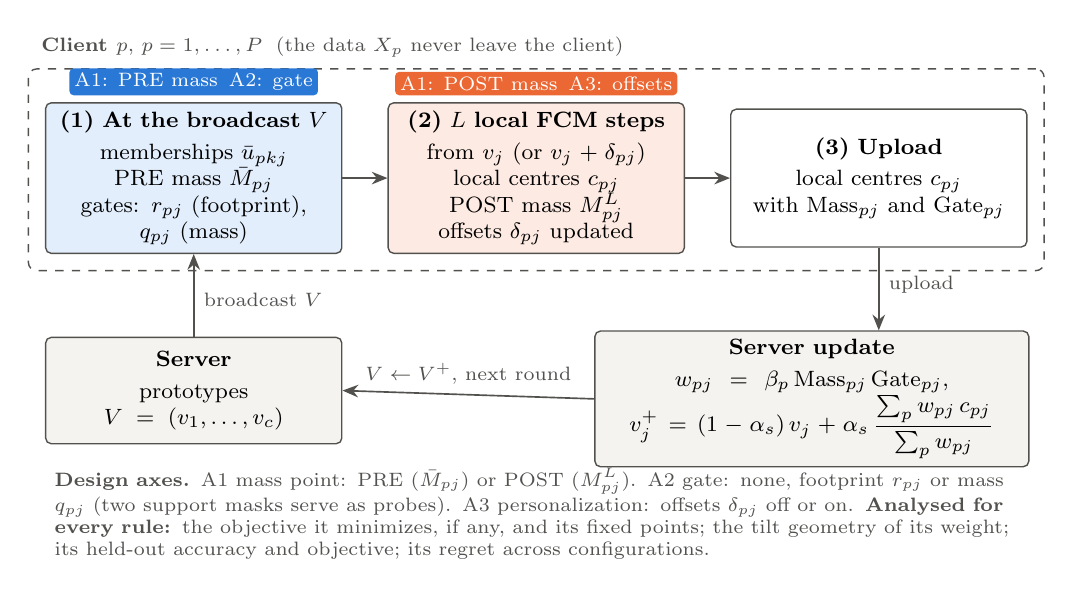
\begin{tikzpicture}[font=\footnotesize, >={Stealth[length=2.0mm,width=1.6mm]},
  box/.style={draw=inktwo, rounded corners=2pt, line width=0.5pt, align=center, inner sep=3pt, fill=white},
  stage/.style={box, text width=3.55cm, minimum height=1.75cm},
  tag/.style={rounded corners=1.5pt, inner sep=1.8pt, font=\scriptsize, text=white, align=center},
  flow/.style={->, line width=0.6pt, draw=inktwo},
  lab/.style={font=\scriptsize, text=inktwo, align=center}]

% ---------------- client: three stages left to right
\node[stage, fill=lblue] (s1) at (0,0)
  {\textbf{(1) At the broadcast $V$}\\[2pt]
   memberships $\bar u_{pkj}$\\ PRE mass $\bar M_{pj}$\\ gates: $r_{pj}$ (footprint),\\ $q_{pj}$ (mass)};
\node[stage, fill=lorange] (s2) at (4.35,0)
  {\textbf{(2) $L$ local FCM steps}\\[2pt]
   from $v_j$ (or $v_j+\delta_{pj}$)\\ local centres $c_{pj}$\\ POST mass $M^{L}_{pj}$\\ offsets $\delta_{pj}$ updated};
\node[stage] (s3) at (8.7,0)
  {\textbf{(3) Upload}\\[2pt]
   local centres $c_{pj}$\\ with $\mathrm{Mass}_{pj}$ and $\mathrm{Gate}_{pj}$};
\draw[flow] (s1) -- (s2);
\draw[flow] (s2) -- (s3);
\node[tag, fill=vblue, anchor=south] at ($(s1.north)+(0,0.08)$) {A1: PRE mass\enspace A2: gate};
\node[tag, fill=vorange, anchor=south] at ($(s2.north)+(0,0.08)$) {A1: POST mass\enspace A3: offsets};
\begin{scope}[on background layer]
  \node[draw=inktwo, dashed, rounded corners=3pt, line width=0.5pt, fit=(s1)(s2)(s3), inner xsep=6pt,
        inner ysep=9pt, yshift=3pt] (client) {};
\end{scope}
\node[lab, anchor=south west] at ($(client.north west)+(0.05,0.02)$)
  {\textbf{Client $p$}, $p=1,\dots,P$ \;(the data $X_p$ never leave the client)};

% ---------------- server row below
\node[box, text width=3.55cm, minimum height=1.35cm, fill=soft, anchor=north] (server) at ($(s1.south)+(0,-1.05)$)
  {\textbf{Server}\\[2pt] prototypes $V=(v_1,\dots,v_c)$};
\node[box, text width=5.3cm, minimum height=1.35cm, fill=soft, anchor=north] (agg) at ($(s3.south)+(-0.85,-1.05)$)
  {\textbf{Server update}\\[2pt]
   $w_{pj}=\beta_p\,\mathrm{Mass}_{pj}\,\mathrm{Gate}_{pj}$,\quad
   $v_j^{+}=(1-\alpha_s)\,v_j+\alpha_s\,\dfrac{\sum_{p}w_{pj}\,c_{pj}}{\sum_{p}w_{pj}}$};
\draw[flow] (server.north) -- node[lab, right, pos=0.45] {broadcast $V$} (s1.south);
\draw[flow] (s3.south) -- node[lab, right, pos=0.45] {upload} (s3.south |- agg.north);
\draw[flow] (agg.west) -- node[lab, above] {$V\leftarrow V^{+}$, next round} (server.east);

% ---------------- axes and analysis layers
\node[lab, anchor=north west, text width=12.45cm, align=left] at ($(server.south west)+(0,-0.18)$)
  {\textbf{Design axes.} A1 mass point: PRE ($\bar M_{pj}$) or POST ($M^{L}_{pj}$).\enspace
   A2 gate: none, footprint $r_{pj}$ or mass $q_{pj}$ (two support masks serve as probes).\enspace
   A3 personalization: offsets $\delta_{pj}$ off or on.\enspace
   \textbf{Analysed for every rule:} the objective it minimizes, if any, and its fixed points; the tilt geometry
   of its weight; its held-out accuracy and objective; its regret across configurations.};
\end{tikzpicture}
\end{document}
